\providecommand{\main}{../../..}
\documentclass[\main/dresen_thesis.tex]{subfiles}
\renewcommand{\thisPath}{\main/chapters/theoreticalBackground/scattering}
\begin{document}
\section{Scattering}\label{sec:theoreticalBackground:scattering}
Scattering describes the general physical process, where radiation changes its straight path due to interaction with another object.
In a broad perspective this includes all various types of radiation - light, x-ray, electron, neutron, \etc .
For example it includes the very daily process of seeing, where after a light wave is emitted from a source like the sun or a light bulb, the wave is scattered from an object in the room before it is finally detected within ones eye.
And scattering also includes the process where after a neutron is generated in a nuclear reactor, it interacts with a sample in a experimental hall before it is measured with a sophisticated detector.

In this work, multiple x-ray and neutron scattering techniques are applied to study the nuclear and magnetic structure of nanoparticles and their manufactured assemblies.
To understand the rich information that is obtained by those techniques, \refsec{sec:theoreticalBackground:scattering:scatteringTheory} presents in the following a brief introduction to the general scattering theory and \refsec{sec:theoreticalBackground:scattering:interactionWithMatter} to the interaction of x-ray and neutrons with matter.
Then the theory behind the mainly applied techniques are discussed: small-angle scattering in \refsec{sec:theoreticalBackground:scattering:SASNanoparticles}, grazing-incidence small-angle scattering in \refsec{sec:theoreticalBackground:scattering:GISAS} and reflectometry in \refsec{sec:theoreticalBackground:scattering:reflectometry}.
\subsection{Scattering Theory}\label{sec:theoreticalBackground:scattering:scatteringTheory}
In general, scattering theory describes the scattering of particles, \textit{e.g.} neutrons or x-ray photons, from a scattering center as depicted in \reffig{fig:theoreticalBackground:scattering:scatteringTheory:scatteringProcess}. An incoming wave $\vec{k}_i$ with defined direction can interact with a scattering center and due to this deviate from its straight path, exiting as outgoing wave $\vec{k}_o$.
If energy is conserved ($|\vec{k}_i| = |\vec{k}_o|$) the process is called elastic and otherwise inelastic.
The vector describing the change from one momentum to the other is noted by
\begin{align}
  \vec{q} \eq \vec{k}_o - \vec{k}_i.
\end{align}
For an elastic process the magnitude of $\vec{q}$ is directly determined by the wavelength $\lambda$ and angle $2\theta$ between $\vec{k}_i$ and $\vec{k}_o$ by
\begin{align}
  |\vec{q}| \eq \frac{4 \pi}{\lambda} \sin(\theta),
\end{align}
where it is used that $|\vec{k}_i| \eq |\vec{k}_o| \eq k \eq \frac{2 \pi}{\lambda}$.

\begin{figure}[tb]
  \centering
  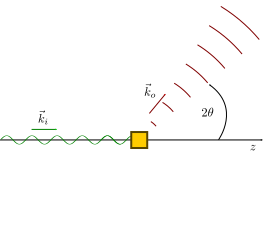
\includegraphics{scatteringTheory_scatterProcess}
  \caption{\label{fig:theoreticalBackground:scattering:scatteringTheory:scatteringProcess}General scattering process. An incoming wave with wave vector $\vec{k}_i$ (green) interacts with a scattering center (yellow) and produces an outgoing wave with wave vector $\vec{k}_o$ (red).}
\end{figure}

Scattering theory determines the transition probabilities for an particle to go from an incoming state to an outgoing state - respectively defined by their energy, momentum and polarization - in dependence of the properties of the particles, the scattering center and their interaction potential.
Thereby it provides a method to calculate from a model the expected scattering intensity, which can be compared to an actual scattering experiment.
In non-relativistic physics, \textit{e.g.} for neutrons, the problem that needs to be solved for this is the Schr\"odinger equation
\begin{align}
  \label{eq:theoreticalBackground:scattering:scatteringTheory:schrodingerEquation}
  \bigg(\frac{\hat{p}^2}{2m} + V \bigg) \ket{\psi} \eq E \ket{\psi},
\end{align}
with the boundary condition $V(\vec{r}) \eq 0$ for $\vec{r}$ outside the scattering region.
For electromagnetic waves such as x-rays, the propagation and interaction with matter is described best by quantum electrodynamics.
For most cases, classical electrodynamics is however sufficient and in \refapp{ch:appendix:calculations:scatteringTheoryElectromagneticWaves} it is shown that the scattering theory from Maxwell's equations maps to the same type of problem as is discussed in the following for the Schr\"odinger equation.

In scattering theory, it is assumed that the scattering particles are non-interacting among themselves, which is a well approximation for photons and neutrons.
The interaction between the wave and the scattering center is described completely by $V(\vec{r})$ and is discussed in further detail in \refsec{sec:theoreticalBackground:scattering:interactionWithMatter}.
To solve \refeq{eq:theoreticalBackground:scattering:scatteringTheory:schrodingerEquation}, the Hamiltonian is defined as
\begin{align}
  H_0 &\eq \frac{\hat{p}^2}{2m},\\
  H &\eq H_0 + V,
\end{align}
and $\ket{\phi}$ is defined as the eigenstates of the free Schr\"odinger equation
\begin{align}
  H_0 \ket{\phi} &\eq E \ket{\phi}.\\
\end{align}
Now, naively, the Schr\"odinger equation can be rearranged as
\begin{align}
  \ket{\psi} &\eq \frac{1}{E - H_0} V \ket{\psi},
\end{align}
but this would not fulfil the boundary condition for $r \rightarrow \infty$, where $V\eq0$, and it has an ill-defined denominator for the eigenstates.
Therefore, the correct solution needs the addition of the free particle solution and a definition how the pole is supposed to be treated.
The latter is done by adding a infinitely small and positively complex value $i\epsilon$ to the denominator. The resulting equation
\begin{align}
  \ket{\psi} &\eq \ket{\phi} +  \frac{1}{E - H_0 + i \epsilon} V \ket{\psi},
\end{align}
is known as the Lippmann-Schwinger equation and  it solves the Schr\"odinger equation by construction.
In position space, it reads as integral equation
\begin{align}
  \psi (\vec{r}) &\eq \phi(\vec{r}) + \int \dint \vec{r}^\prime \bra{\vec{r}}\frac{1}{E - H_0 + i \epsilon} \ket{\vec{r}^\prime} V (\vec{r}^\prime)\psi (\vec{r}^\prime),
  \label{eq:theoreticalBackground:scattering:scatteringTheory:LippmanSchwingerIntegralEquation}
\end{align}
where it is used that the single-particle potential is diagonal in position space $\bra{\vec{r}} V \ket{\vec{r}^\prime} = V(\vec{r}) \delta(\vec{r} - \vec{r}^\prime)$.
The simplest solution for the free Hamiltonian is given by a plane wave
\begin{align}
  \phi_{\vec{k}}(\vec{r}) \eq e^{i\vec{k} \cdot \vec{r}}.
\end{align}
As a plane wave extends infinitely in space with constant amplitude, plane waves are not normalizable.
To describe physical particles with finite width, a superposition of plane waves can be used
\begin{align}
  \varphi(\vec{r}) \eq \frac{1}{\sqrt{2 \pi}^3} \int \dint \vec{k} \hat{\varphi} (\vec{k}) \phi_{\vec{k}}(\vec{r}),
\end{align}
where $\hat{\varphi} (\vec{k})$ describes the probability amplitude for a momentum $\vec{k}$ and is essentially the Fourier transform of $\varphi(\vec{r})$.
However, as there is no term that couples momenta $\vec{k}$ and $\vec{k}^\prime$, it is sufficient to solve the Schr\"odinger equation just for a single plane wave and form the wave packet in the end.

The matrix element within the integral equation \refeq{eq:theoreticalBackground:scattering:scatteringTheory:LippmanSchwingerIntegralEquation} can be solved straight-forward in momentum space using the residue theorem as shown in \refapp{ch:appendix:calculations:greenFunctionFreeHamiltonian} and results in
\begin{align}
  \bra{\vec{r}}\frac{1}{E - H_0 + i \epsilon} \ket{\vec{r}^\prime} \eq -\frac{m}{2 \pi \hbar^2} \frac{e^{ik|\vec{r} - \vec{r}^\prime|}}{|\vec{r} - \vec{r}^\prime|}.
\end{align}
Thus the integral representation of the Lippmann-Schwinger equation is
\begin{align}
  \psi (\vec{r}) &\eq e^{i\vec{k}_i \cdot \vec{r}} - \frac{m}{2 \pi\hbar^2} \int \dint \vec{r}^\prime \frac{e^{ik|\vec{r} - \vec{r}^\prime|}}{|\vec{r} - \vec{r}^\prime|} V (\vec{r}^\prime)\psi (\vec{r}^\prime).
\end{align}
The resulting wave function can be nicely interpret as a sum of the incoming plane wave and the scattered wave, which is itself a superposition of spherical waves generated at $\vec{r}^\prime$ and that is modulated by the interaction potential $V(\vec{r}^\prime)$ and the wave field at this point.

In a standard experimental setup, the detector is usually at a position that is considerably far away on a length scale relative to the scattering volume $r^\prime \ll r$.
Therefore a good approximation and large simplification in calculation is
\begin{align}
  |\vec{r} - \vec{r}^\prime| \eq& r - \frac{\vec{r} \cdot \vec{r}^\prime}{r} + \mathcal{O}\bigg(\frac{{r^\prime}^2}{r}\bigg),\\
  \frac{1}{|\vec{r} - \vec{r}^\prime|} \eq& \frac{1}{r} + \mathcal{O}\bigg(\frac{r^\prime}{r^2} \bigg),\\
  \vec{k}_o \eq& k \vec{r} / r,
\end{align}
where the latter reads that as the detector is far away relative to the sample size, the outgoing wave points essentially into the direction of the detector.
Then the Lippmann-Schwinger equation reads
\begin{align}
  \psi (\vec{r}) &\eq e^{i\vec{k}_i \cdot \vec{r}} - \frac{m}{2 \pi\hbar^2} \frac{e^{ikr}}{r} \int \dint \vec{r}^\prime e^{-i\vec{k}_o \cdot \vec{r}^\prime} V (\vec{r}^\prime)\psi (\vec{r}^\prime),
\end{align}
and the scattered wave only reads as a single spherical wave $e^{ikr} / r$ with an amplitude determined by the interaction of the wave function with the scattering center potential.

The Lippmann-Schwinger equation can be used to solve the scattering problem for any potential $V$ iteratively by starting on the right hand side of the equation with the free particle solution for $\psi (\vec{r})$ and then recursively inserting the solution back into the Lippmann-Schwinger equation, \etc.
The first iteration
\begin{align}
  \psi (\vec{r}) &\eq e^{i\vec{k}_i \cdot \vec{r}} - \frac{m}{2 \pi\hbar^2} \frac{e^{ikr}}{r} \int \dint \vec{r}^\prime e^{-i\vec{q} \cdot \vec{r}^\prime} V (\vec{r}^\prime),
  \label{eq:theoreticalBackground:scattering:scatteringTheory:firstBornApproximation}
\end{align}
is known as the Born approximation and is the starting point for many further calculations. It fully describes the case where the wave undergoes only a single scattering event as it passes through the sample.

Finally, the flux of scattered particles to a solid angle $\dint \Omega$ for a given incoming flux of particles is determined from the wave function, which is an experimentally accessible quantity that can be measured with a detector.
The probability current of a wave function $\psi$  is calculated in quantum mechanics by
\begin{align}
  \vec{j} \eq \frac{\hbar}{2mi} \bigg( \psi^* \vec{\nabla} \psi - \psi \vec{\nabla} \psi^* \bigg).
\end{align}
Thus the incoming current and scattered current is evaluated to be
\begin{align}
  \vec{j}_i &\eq \frac{\hbar \vec{k}_i}{m}\\
  \vec{j}_o &\eq \bigg| \frac{m}{2 \pi\hbar^2} \int \dint \vec{r}^\prime e^{-i\vec{q} \cdot \vec{r}^\prime} V (\vec{r}^\prime) \bigg|^2 \frac{\hbar k}{m r^2} \hat{r} + \mathcal{O} \bigg(\frac{1}{r^3}\bigg),\\
\end{align}
and with this the incoming flux per unit area is determined to $\Phi_i \eq \vec{j}_i \cdot \hat{k}$, and the scattered flux per surface area to $\Phi_o \eq \vec{j}_o \cdot \dint \vec{S}$, where $\dint \vec{S} \eq r^2 \dint \Omega \hat{r}$.
Experimentally, the flux of scattered particles to a solid angle is measured and normalized to the corresponding flux of incoming particles. This ratio is known as the differential cross section and plugging in the previous results, it is calculated in Born approximation via
\begin{align}
  \frac{\dint \sigma}{\dint \Omega} \eq \frac{\Phi_o}{\Phi_i \dint \Omega} \eq \bigg| \frac{m}{2 \pi\hbar^2} \int \dint \vec{r}^\prime e^{-i\vec{q} \cdot \vec{r}^\prime} V (\vec{r}^\prime) \bigg|^2.\label{eq:theoreticalBackground:scattering:scatteringTheory:differentialCrossSectionIntegralOverPotential}
\end{align}

\subsection{Interaction of X-rays and Neutrons with Matter}\label{sec:theoreticalBackground:scattering:interactionWithMatter}
To calculate the differential cross section, it is necessary to know how the scattering wave and the sample interact with each other, which is represented by the potential $V$.
Even though in the previous chapter, the differential cross section is derived for quantum mechanical particles, it is shown in \refapp{ch:appendix:calculations:scatteringTheoryElectromagneticWaves} that a similar formula results for x-rays from classical electrodynamics.
In the case of x-rays, the dominant coupling to consider is the electromagnetic interaction of the x-ray photons with the electron shells of the atoms making up the material.
When an electron cloud is considered to oscillate in phase with the incoming x-ray, the differential cross section is modelled as
\begin{align}
  \frac{\dint \sigma}{\dint \Omega} \eq |\hat{e}_i \cdot \hat{e}_f|^2 \biggl| \int \dint V e^{-i \vec{q} \cdot \vec{r}}  r_e \rho_e (\vec{r}) \biggr|^2.
\end{align}
Here $|\hat{e}_i \cdot \hat{e}_f|^2$ is a polarization factor depending on the geometry and the source of the experiment, $r_e \approx 2.8 \unit{fm}$ is the classical electron radius and $\rho_e$ the density distribution of the electron cloud.
This result is known as Thomson scattering.
In general the electronic structure and response of materials is very complex and highly dependant on the energy of the incoming photon.
In the derivation of the formula above it is assumed that the electron cloud follows the incoming wave via Newton's law $\vec{F} \eq m \vec{a} \eq -e\vec{E}$.
This neglects resonance, absorption and dispersion effects.
Those become important whenever the energy of x-ray is close to electronic transitions in the material or is high enough that it  ejects electrons from their respective positions.
However in the frame of this work, such effects are negligible and further discussions about it can be found in literature \cite{AlsNielsen_2011_Eleme}.

For neutrons on the other hand, two fundamental interactions with a material exist.
On the one hand the neutron scatters via the short-ranged residual strong interaction with the atomic nuclei and on the other the magnetic moment of the neutron contributes to a scattering via the electromagnetic interaction with the internal magnetic field of the sample.
For the nuclear scattering, the length scale of the residual strong force is on the order of $\mathcal{O} (10^{-15} \unit{m})$, whereas the wavelength of thermal neutrons $\mathcal{O} (10^{-10} \unit{m})$ is much larger.
The nucleus can therefore be considered point-like and the potential for the scattering of a free neutron from a collection of nuclei positioned at $\vec{r}_j$ can be modelled by a sum of Fermi pseudopotentials
\begin{align}
  V(r) \eq \frac{2 \pi \hbar^2}{m} \sum_j b_j \delta(\vec{r} - \vec{r}_j),\label{eq:theoreticalBackground:scattering:scatteringTheory:neutronScatteringPotentialSum}
 \end{align}
where $b$ is the bound scattering length for said nucleus, which is different for every element and isotope and therefore includes the  information to differentiate between them.
The \textit{ab initio} calculation of the scattering length for an isotope is a hard task, due to the complicated nature of the strong force, which is described by the theory of quantum chromodynamics, and needs detailed knowledge of the subatomic structure.
However, the experimental values of the bound scattering length have been tabulated for most isotopes and can be combined to model an investigated material of known composition \cite{Sears_1992_Neutr}.
The bound scattering length is in general a complex number $b \eq b^\prime - i b^{\prime \prime}$, where the complex part describes neutron absorption due to nuclear reactions.
Furthermore the bound scattering length comprises a coherent $b_c$ and incoherent $b_i$ cross section, where the incoherent cross section depends on the relative orientation of the neutron spin $\vec{s}$ to the nucleus angular momentum $\vec{I}$
\begin{align}
  b \eq b_c + \frac{2 b_i}{\sqrt{I(I+1)}} \vec{s} \cdot \vec{I}.
\end{align}
In the frame of the experiments and materials discussed in this thesis, neutron absorption by the material can be neglected.
Also, the orientation of the nuclei angular momentum relative to the neutron spin can be considered random and therefore the incoherent scattering contains no information about the structure of the samples but is a constant background.
When the exact atomic structure is not of interest, the continuum limit can be taken for the sum in \refeq{eq:theoreticalBackground:scattering:scatteringTheory:neutronScatteringPotentialSum} and it can be replaced by a scattering length density
\begin{align}
  \sum_j b_j \delta(\vec{r} - \vec{r}_j) \rightarrow \rho(\vec{r}),
\end{align}
where the value of $\rho(\vec{r})$ is determined by summing over the bound scattering lengths of all atoms in a unit cell of volume $V_{uc}$ for a given material at position $\vec{r}$
\begin{align}
  \rho(\vec{r}) \eq \frac{1}{V_{uc}} \sum_i^n b_i.
\end{align}
The differential cross section is thus obtained for neutrons from evaluating
\begin{align}
  \frac{\dint \sigma}{\dint \Omega} \eq \bigg| \int \dint \vec{r} e^{-i\vec{q} \cdot \vec{r}} \rho (\vec{r}) \bigg|^2.
  \label{eq:theoreticalBackground:scattering:scatteringTheory:differentialCrossSectionBornApproximation}
\end{align}
It is interesting to note here that for x-rays, up to the polarization factor, the same formula applies when the x-ray scattering length density is identified from the electron density as $\rho \eq r_e \rho_e$.
Therefore, every following discussion starting from this equation includes both the scattering of x-rays from the electron clouds of matter and the scattering of neutrons from the nuclear structure.

The magnetic scattering of neutrons from the magnetic structure of the material can be included by adding a Zeeman potential to the Hamiltonian
\begin{align}
  V_m (\vec{r}) \eq - \vec{\mu}_n \cdot \vec{B},
\end{align}
where $\vec{\mu}_n \eq \mu_n \hat{\sigma}$ is the magnetic moment of the neutron, which has a magnitude of $\mu_n \eq 9.662 \cdot 10^{-27} \unit{JT^{-1}}$, and is quantum mechanically given by the spin operator $\hat{\sigma}$, and $\vec{B}$ is the magnetic field generated by the sample due to the bound electron orbital motion and spins.
In \refapp{ch:appendix:calculations:magneticScatteringTheory} it is derived that the contribution by the spin to the differential cross section can be modelled similar to the nuclear scattering as Fourier transform over a magnetic scattering length density
\begin{align}
  f_M (\vec{q}) \eq & \hat{\mu}_n \cdot \hat{s}_\perp \int \dint \vec{r} e^{- i \vec{q} \cdot \vec{r}} \rho_\mathrm{mag}(\vec{r}),
\end{align}
where the magnetic scattering length density is defined by the spin density as
\begin{align}
  \rho_\mathrm{mag} (\vec{r}) \eq \frac{m_n}{\hbar^2}  \frac{\mu_0}{2\pi} \mu_B \mu_n s_e (\vec{r}),
\end{align}
and an additional prefactor $\hat{\mu}_n \cdot \hat{s}_\perp$, where $\hat{s}_\perp$ is the fraction of the spins that are directed in the plane perpendicular to the scattering vector $\vec{q}$.
Thus, polarized neutron scattering allows to measure the spin density of a sample in that plane.

The polarization of the incoming neutron beam in an experiment is defined and stabilized by a weak magnetic guide field.
When $\hat{s}_\perp$ is parallel (antiparallel) to this direction, $f_M$ contributes with a positive (negative) sign to the differential cross section and the direction of the spin is conserved during the scattering.
On the other hand, when $\hat{s}_\perp$ is perpendicular to this direction, the spin operator results in a flip of the neutron spin during the scattering.
This allows, through careful analysis of the non-spin flip and spin flip channels, to measure additionally the direction of the magnetization in the plane perpendicular to the scattering vector.



\subsection{Coherence \& Instrumental Resolution}\label{sec:theoreticalBackground:scattering:CoherenceInstrumentalResolution}
In the derived theory, x-ray and neutrons are infinitely extending plane waves of a single wavelength $\lambda$ and the complete sample is radiating spherical waves in phase with the incoming wave with the scattering angle $\theta$.
In reality, however, the beam has a finite width defined by collimation, which leads to a divergence of the beam of $\Delta \theta$ and the beam is not perfectly monochromatic, but has a finite distribution of wavelengths $\Delta \lambda$.
This leads to a superposition of multiple patterns in a real experiment and possibly to a loss of information due to the finite instrumental resolution that destroys the interference pattern.
To quantify what area of the sample is radiating in phase, such that the interference is not destroyed, the coherence of the beam needs to be evaluated.

The wavelength spread $\Delta \lambda$ defines the longitudinal (or temporal) coherence of the beam. It can be quantified by considering on which length scale $L_L \eq n \lambda$ two waves with wavelengths $\lambda$ and $\lambda + \Delta \lambda$ start to interfere destructively
\begin{align}
  n\lambda \eq& \biggl(n - \frac{1}{2} \biggr)(\lambda + \Delta \lambda),
\end{align}
which can be rearranged to
\begin{align}
  L_L \eq& \frac{\lambda}{2} \biggl(1 + \frac{\lambda}{\Delta \lambda} \biggr) \approx \frac{\lambda^2}{2 \Delta \lambda},
\end{align}
where $\Delta \lambda / \lambda$ is typically in the order of $5\, \%$ for neutron experiments, which means the longitudinal coherence length is for neutrons with wavelength $\lambda \eq 5 \angstrom$ in the order of $L_L \eq 50 \angstrom$.

The finite beam size results in a transversal coherence, which destroys the interference pattern when the angular separation $\Delta \theta$ leads to a destructive interference for the wavelength $\lambda$ on the length scale $L_T$
\begin{align}
  L_T \eq \frac{\lambda}{2 \Delta\theta}.
\end{align}
The transversal coherence length might be different in the horizontal and vertical plane and depends strongly on the experimental geometry.
It depends on the chosen slits and distances between the slits, sample and detector.
For a typical beam divergence in the order of $\delta \theta \eq 0.3^\circ$, a transversal coherence length of $L_T \eq 500 \angstrom$ is obtained for $\lambda \eq 5 \angstrom$.

The three coherence length scales define a coherence volume, for which a sample radiates in phase and produces interference pattern.
This has to be kept in mind when designing models for the evaluation of scattering experiments, as over larger length scales the contributions add incoherently, and instead of the amplitudes, the intensities need to be added.

To include furthermore the smearing of the intensities due to the wavelength spread and beam divergence, an effective spread in the wave vector is obtained by error propagation
\begin{align}
  \frac{\Delta q}{q} \eq \sqrt{\biggl( \frac{\Delta \lambda}{\lambda} \biggr)^2 + \biggl( \cot (\theta) \Delta \theta \biggr)^2}.
\end{align}
The effective smearing is modelled by a Gaussian function with width $\Delta q$ that is convoluted with the calculated model of the differential cross section for a given $q$ range.

\subsection{Small-Angle Scattering from Nanoparticles}\label{sec:theoreticalBackground:scattering:SASNanoparticles}
Small-angle scattering is a technique to study nanometer sized objects when the wavelength of the scattered particle is in the order of a few {\aa}ngstr\"om.
Here, the forward scattering of a collimated beam through a sample is measured on a position sensitive detector around an opening angle in the order of $2 \theta \eq 0.1^\circ - 10^\circ$.
As the magnitude of the scattering vector $q$ is proportional to $\sin(\theta)$ and $q$ is inversely proportional to the probed length scale, smaller scattering angles $\theta$ mean that larger length scales are probed.
At the considered length scales, the atomic structure of the materials can be treated in the continuum limit as described in \refsec{sec:theoreticalBackground:scattering:interactionWithMatter}.

\begin{figure}[tb]
  \centering
  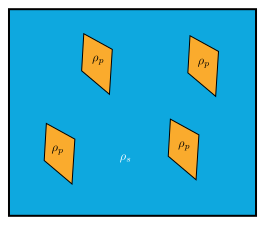
\includegraphics{scatteringTheory_sasParticlesInSolvent}
  \caption{\label{fig:theoreticalBackground:scattering:scatteringTheory:sasParticlesInSolvent}Scattering length density described in \refeq{eq:theoreticalBackground:scattering:scatteringTheory:sasParticlesInSolvent}. The space is completely filled with the solvent $\rho_s$ and at positions of the nanoparticles the solvent is replaced by the scattering length density function describing a nanoparticle $\rho_p$.}
\end{figure}
In the following, the application of small-angle scattering to the study of nanoparticles in dispersion is described.
In a first step, a dispersion that consists of monodisperse and equally oriented nanoparticles is considered.
In this case the scattering length density is modelled by a constant background value given by the solvent $\rho_s$ and parts where the solvent is replaced by the nanoparticles.
As every particle is equally oriented and of same shape, this is included by summing over a function $\rho_p (\vec{r})$ that contains the complete description of shape and composition of a single particle and which is shifted to the different center positions $\vec{r}_i$ of the nanoparticles
\begin{align}
  \rho(\vec{r}) \eq& \rho_s + \sum_{i=1}^N \Delta \rho_{p}(\vec{r} - \vec{r}_i).\label{eq:theoreticalBackground:scattering:scatteringTheory:sasParticlesInSolvent}
\end{align}
The nanoparticle scattering length density can be written as convolution of a function $\rho_{p}(\vec{r})$, which describes the shape and composition of a single nanoparticle, and a function $s(\vec{r})$ describing the position of $N$ nanoparticles in the solvent\footnote{The convolution of two functions is defined as $(f*g)(x) \eq \int \dint \tau f(\tau) g(x-\tau)$.
 When $f$ is a sum over $\delta$ functions, the convolution operation generates a sum of the function $g$, centred at every grid point defined by the $\delta$ functions
\begin{equation}
  \int \dint \tau \sum_{i=1}^N \delta(\tau - x_i) g(x-\tau) \eq \sum_{i=1}^N g(x - x_i).
\end{equation}}
\begin{align}
  \rho(\vec{r}) \eq& \rho_s + (s * \Delta \rho_{p})(\vec{r}),\\
  s(\vec{r}) \eq& \sum_{j=1}^N \delta(\vec{r} - \vec{r}_j).
\end{align}

The macroscopic differential cross section, which is the differential cross section scaled to the integrated volume
\begin{align}
  \frac{\dint \Sigma}{\dint \Omega} \eq \frac{1}{V} \frac{\dint \sigma}{\dint \Omega},
\end{align}
can then be evaluated in the Born approximation by inserting the scattering length density in \refeq{eq:theoreticalBackground:scattering:scatteringTheory:differentialCrossSectionBornApproximation}
\begin{align}
  \frac{\dint \Sigma}{\dint \Omega}
  \eq& \frac{1}{V} \bigg| \int_V \dint \vec{r}^\prime e^{-i\vec{q} \cdot \vec{r}^\prime} \rho (\vec{r}^\prime) \bigg|^2 \\
  \eq& \frac{1}{V} \bigg| \int_{V} \dint \vec{r}^\prime e^{-i\vec{q} \cdot \vec{r}^\prime} \biggl( s * \Delta \rho_{p}) \biggr) (\vec{r}^\prime) + \underbrace{\int_{V} \dint \vec{r}^\prime e^{-i\vec{q} \cdot \vec{r}^\prime} \rho_s }_{(2 \pi)^3 \delta(\vec{q}) \rho_s} \bigg|^2.
\end{align}
The integral over the constant solvent scattering length density is evaluated to zero for $\vec{q} \neq 0$.
The case of $\vec{q} \eq 0$ corresponds to forward scattering, which is not studied in small-angle scattering as the direct beam is in most experiments blocked to protect the detector.

The convolution theorem turns the remaining integral to a product of two integrals
\begin{align}
  \frac{\dint \Sigma}{\dint \Omega}
  \eq \frac{N}{V} \underbrace{\frac{1}{N} \bigg|\int \dint \vec{r} e^{-i\vec{q} \cdot \vec{r}} s(\vec{r})\bigg|^2}_{S(\vec{q})}
  \underbrace{ \bigg|\int_{V_{p}} \dint \vec{r} e^{-i\vec{q} \cdot \vec{r}} (\rho_p (\vec{r}) - \rho_s) \bigg|^2}_{P(\vec{q})},\label{eq:theoreticalBackground:scattering:scatteringTheory:sasParticlesformStructureFactor}
\end{align}
The first integral is called the structure factor $S(\vec{q})$ and the second the form factor $P(\vec{q})$.
The form factor describes the scattering due to the shape and properties of a single nanoparticle.
In the definition of the volume integral for the form factor, it is enough to integrate over the volume of a single particle $V_p$ as the integrand is $0$ outside, and $\Delta \rho_p (\vec{r})$ is explicitly written.
The integral, before applying the magnitude square, is called the form factor amplitude and is denoted by a lower case $p(\vec{q})$.
As the magnitude removes the phase of the amplitude, it's in general hard to revert the integration and conclude from the differential cross section directly on the shape and composition of the nanoparticle due to the missing information.
Using additional information from multiple experiments a model can, however, be formulated for a particle and from this the form factor can always be calculated, which is compared to the small-angle scattering experiment for confirmation.

The structure factor in \refeq{eq:theoreticalBackground:scattering:scatteringTheory:sasParticlesformStructureFactor} modulates the scattering due to the relative positions of the ensemble of individual nanoparticles.
It is normalized to the number of particles $N$ for proper scaling behaviour and can generally be further discussed by inserting the definition of the function $s(\vec{r})$
\begin{align}
  S(\vec{q}) &\eq \frac{1}{N} \bigg| \sum_j  e^{-i\vec{q} \cdot \vec{r}_j} \bigg|^2\\
  &\eq \frac{1}{N}  \bigg( \sum_j  e^{-i\vec{q} \cdot \vec{r}_j} \bigg) \bigg( \sum_k  e^{i k\vec{q} \cdot \vec{r}_k} \bigg)\\
  &\eq \frac{1}{N}  \sum_{j, k}  e^{-i\vec{q} \cdot (\vec{r}_j - \vec{r}_k) }\\
  &\eq 1 + \frac{1}{N}  \sum_{j \neq k}  e^{-i\vec{q} \cdot (\vec{r}_j - \vec{r}_k)},
\end{align}
where in the last step the sum over all indices, where $j=k$, was performed.
At this point, specific models of the relative nanoparticle positions needs to be looked at for further discussion.

The simplest models that can be solved are perfectly ordered crystals and disordered liquids.
For ordered crystals, constructive contributions are found when $\vec{q} \cdot (\vec{r}_j - \vec{r}_k) \eq 2 \pi n$, which is Bragg's law in this frame.
In the case of dilute dispersions, the sum is over random phases and vanishes due to the pre factor, resulting in $S(\vec{q}) = 1$.
This case is most often the desired one in a small-angle scattering experiment on nanoparticles as it eliminates the need to model a structure factor.
Therefore, in a experiment, the sample is diluted such that the structure factor is approximately $1$, but the measured intensity is still strong enough to be counted in a reasonable amount of measurement time.
In this case, only the form factor $P(\vec{q})$ for a specific sample needs to be modelled

For a form factor, the simplest to solve model of a nanoparticle is that of a sphere due to it's high symmetry.
The scattering length density is then just a constant within the volume of the sphere and the form factor $P_\mathrm{sph}$ can be solved analytically to
\begin{align}
  P_\mathrm{sph} (\vec{q})
  \eq & \bigg|\int_{V_{p}} \dint \vec{r} e^{-i\vec{q} \cdot \vec{r}} (\rho_p - \rho_s) \bigg|^2 \\
  \eq & \bigg|(\rho_p - \rho_s) \int_0^R \dint r \int_0^{2 \pi} \dint \phi \int_0^\pi \dint \theta r^2 \sin(\theta) e^{-i q r \cos(\theta)}  \bigg|^2 \\
  \eq &  \bigg| 4\pi R^3 (\rho_p - \rho_s) \frac{\sin(qR) - qR\cos(qR)}{(qR)^3}  \bigg|^2\\
  \eq & V_\mathrm{sph}^2 (\rho_p - \rho_s)^2 \bigg|3 \frac{\sin(qR) - qR\cos(qR)}{(qR)^3}  \bigg|^2,
\end{align}
where $V_\mathrm{sph}$ is the volume of the sphere.
Thus, the macroscopic differential cross section for diluted nanospheres in a solvent is
\begin{align}
  \frac{\dint \Sigma}{\dint \Omega}
  \eq \alpha V_\mathrm{sph} (\rho_p - \rho_s)^2 \bigg|3 \frac{\sin(qR) - qR\cos(qR)}{(qR)^3}  \bigg|^2,
\end{align}
with $\alpha \eq NV_\mathrm{sph} / V$ the volume concentration of the particles in the solvent.
The result shows the typical dependence of the differential cross section on the particle concentration, volume and contrast to the solvent.
The latter is especially used for contrast variation techniques in neutron scattering, where solvents (especially $\mathrm{H_2O}$ and $\mathrm{D_2O}$) are mixed to tune the scattering length density of the solvent to enhance the signal or mask particles.
The derivation of further form factors used in this work such as a cube or superball, and how to include multiple compositions in a core shell model is further elaborated in \refapp{sec:appendix:formfactors}.
As will become evident in the following work, small-angle scattering is a very powerful technique to characterize a large number of particles in a sample, and the obtained results are valuable in evaluating higher order experiments which rely on the characterized samples.
\subsection{Reflectometry}\label{sec:theoreticalBackground:scattering:reflectometry}
Nanoparticles that are deposited on a substrate self-assemble to higher order structures under certain conditions that are elaborated in later chapters of this work.
It is of high interest to study the physical properties of the ensemble and whether they differ from the single particle properties and how this depends on the superstructure.
A technique to study the vertical structure of a thin sample on a substrate is reflectometry.
X-ray reflectometry allows to study the average electron density in a sample with depth resolution, whereas neutron reflectometry allows to study the nuclear structure.
Additionally, polarized neutron reflectometry allows to resolve the magnetic density with depth resolution.
The general technique is described in the following in the frame of the study of nanoparticles on a substrate, as it is applied in later parts of this thesis.

\subsection{Grazing Incidence Small-Angle Scattering from a Surface}\label{sec:theoreticalBackground:scattering:GISAS}
Additionally to the vertical structure, it is interesting to study the lateral structure of an ensemble of nanoparticles to obtain the complete 3 dimensional information.
For this purpose grazing-incidence small-angle scattering (GISAS) has proven an efficient technique to measure the off-specular scattering from which in-plane order within a sample can be extracted with high resolution.
As in the case of reflectometry, it is possible to obtain information about the lateral electron density using GISAS with x-rays (GISAXS), and about the lateral nuclear and magnetic structure using (polarized) neutrons (GISANS, polGISANS).
The experimental setup ...

To model the off-specular scattering measured in grazing incidence small angle scattering, the problem can be discussed in distorted wave born approximation (DWBA). Here, the potential $V(\vec{r})$ of a thin layer is decomposed into a sum of the laterally averaged potential $V_1(\vec{r})$ and the in-plane fluctuations $\delta V(\vec{r})$, which are treated as small perturbation $|\delta V| \ll |V_1|$
\begin{align}
  V(\vec{r}) \eq V_1(\vec{r}) + \delta V(\vec{r}).
\end{align}

\end{document}